\documentclass[12pt, a4paper]{article}
\usepackage[brazil]{babel}
\usepackage[utf8]{inputenc}
\usepackage{url}
\usepackage{lscape}
\usepackage{tabularx}
\usepackage{longtable}
\usepackage{setspace}
\usepackage[pdftex]{graphicx}
\usepackage{multicol}
\graphicspath{{./imagens/}}
\usepackage{color}
\usepackage{listings}
\usepackage{amsfonts, amssymb, mathrsfs}
\usepackage{bm}
\usepackage{cite}
\usepackage{changepage}
\usepackage{gensymb}
\usepackage{mathptmx}
\usepackage{pdfpages}
\usepackage[numbib]{tocbibind}
\usepackage{amssymb,amsmath}
\usepackage{algorithmic}
\usepackage[portuguese, ruled, linesnumbered]{algorithm2e}
\usepackage{indentfirst}
\usepackage{blindtext}

\newcommand{\bbeta}{\mbox{\boldmath $\beta$}}
\newcommand{\bxi}{\mbox{\boldmath $\xi$}}
\newcommand{\Y}{\mathbf{Y}}
\newcommand{\X}{\mathbf{X}}
\newcommand{\EM}{\mathcal{E}}

\setlength{\parskip}{2mm}
\usepackage[a4paper,top=2.554cm,bottom=2.554cm,left=2.554cm,right=2.554cm]{geometry} 

\usepackage{natbib} % 
\bibpunct{(}{)}{;}{a}{,}{,}


\usepackage[backend=biber,style=numeric,sorting=none]{biblatex}
\addbibresource{references.bib}


\usepackage[usenames,svgnames,dvipsnames]{xcolor}
\usepackage[font=small,format=plain,labelfont=bf,up,textfont=it,up]{caption}

\usepackage[pdftex,plainpages=false,pdfpagelabels,
linktocpage,
colorlinks=true,
citecolor=blue,
linkcolor=NavyBlue,
urlcolor=DarkRed,
filecolor=green,
bookmarksopen=true,
pdfauthor={Nome do autor do documento},
pdfsubject={subject1, subject2, ...},
pdfkeywords={keyword1, keyword2, ...}
]{hyperref}



\lstset{language=R,
    basicstyle=\small\ttfamily,
    stringstyle=\color{DarkGreen},
    otherkeywords={0,1,2,3,4,5,6,7,8,9},
    morekeywords={TRUE,FALSE},
    deletekeywords={data,frame,length,as,character},
    keywordstyle=\color{blue},
    commentstyle=\color{DarkGreen},
}


\singlespacing  % espa\c{c}amento



\begin{document}


\par

%%%%%%%%%%%%%%%%%%%%%%%%%%%%%%%%%%%%%% CAPA %%%%%%%%%%%%%%%%%%%%%%%%%%%%%%%%%%%%%%%%%%%%%%%%%

\begin{center}

\thispagestyle{empty}

\vspace*{-1.5cm}


\hspace*{-0.1cm} {\rule[-1ex]{16cm}{0.01cm}}
\begin{center}
\hspace{-1cm}
\begin{minipage}[s]{2cm}

\includegraphics[width=2.2cm]{logounicamp.eps}
\end{minipage}
\begin{minipage}[s]{11cm}
{\begin{center} {\LARGE Universidade Estadual de Campinas}\\ \vspace{0.2 cm}
{Instituto de Matem\'{a}tica, Estat\'{\i}stica e Computa\c{c}\~{a}o Cient\'{\i}fica }\\ \vspace{0.1 cm}
{Professor Maicon R. Correa}
\end{center}}
\end{minipage}\begin{minipage}[s]{1 cm}

\includegraphics[width=1.8 cm]{logoimecc.eps}
\end{minipage}
\end{center}

\vspace{3 cm}

{\Large\bf{Análise de algoritmos para resoluções de sistemas lineares}}\\
\Large{\textbf{MS512}}

\vspace{2cm}


\Large{\text{Alexia Pereira Santos 165275}}\\
\Large{\text{Elizabeth Borgognoni Souto 170409}}\\
\Large{\text{Isabella Gomide Alves 175293}}\\
\Large{\text{Tiago Gimenez 177718}}\\
\Large{\text{Vinícius Figueiredo Fernandes 157510}}


\vspace{8cm}

{\small{CAMPINAS}}\\ {\small{2019}}
\end{center}
\hspace*{-0.1cm} {\rule[-1ex]{16cm}{0.01cm}}

\newpage

\section{Introdução}

%a norma ela serve pra ver q auqatidade de erros que o sistema ta dando. Quanto maior o n maior o erro da respota do sistema, e conseguimos ver isso pela inversa e condicionamento 


%%qual metodo p analisa qual meterroeodo tem o menor la norma pra ver se o sistema esta convergindo pra resposta certa 
%e pela inversa verificar se está correto
%o que acontece com os metodos quando colocamos o n muito grande

Os métodos de solução de sistemas lineares estão associados com muitos problemas da engenharia, física e matemática. Nesse estudo, tratamos de técnicas numéricas empregadas para obter a solução desses sistemas. Abordaremos os métodos que abrangem as resoluções dos sistemas lineares com diferentes níveis de eficiências, tais como: fatoração de Cholesky, Gram Schmidt e Householder.

O objetivo é analisar e comparar os métodos supracitados utilizando a matriz de Hilbert como objeto de estudo. A comparação das técnicas é feita a partir do uso da norma 1 e do número de condicionamento associado. Sendo assim, o condicionamento verifica a estabilidade da matriz. O mesmo é calculado pela multiplicação da norma 1 da matriz pela norma 1 da matriz inversa.

%quanto maior o n(dimensão da matriz) 


%um vez que analisamos tal acurácia mediante ao aumento do n (tamanho da matriz) 

\section{Metodologia}

%Como o estudo envole sistemas lineares ($Ax = b$), foram estudados os métodos que são abordados nas subseções seguintes. 

%Foi utilizado o software RStudio para implementar os algoritmos dos  métodos para a analise do condicionamento

%%explicar como cada metodo funciona 

\subsection{Fatoração de Cholesky}

A decomposição de Cholesky procura decompor uma matriz $A$ na forma $A = R^{T}R$,onde $R$ é uma matriz triangular superior com elementos da diagonal principal estritamente positivos. Para tanto, exige-se que a matriz $A$ seja simétrica definida positiva. Para que $A$ seja simétrica definida positiva, $A$ deve ser simétrica e $x^{T}Ax > 0$, para todo $x > 0$.

\noindent
Apresentamos a seguir o pseudo-algoritmo da decomposição de Cholesky.


 \begin{algorithm}
   \SetAlgoLined
   
   \Inicio{
    Se n $>$ 0\\
    \Para{i de 1 até n}{
    \Para{j de 1 até i}{
    soma = 0\\
    \Para{k de i ate j}{
    soma = (soma + $R^{T}_{i,k}$ * $R^{T}_{j,k}$)}\\
    
    \uIf{$A_{i,i}$ menor ou igual a 0}{
    ``saia''}\\
    \uIf{i igual j}{
    $R^{T}_{i,j} = \sqrt{A_{i,i} - soma}$\\}
    \Else{$R^{T}_{i,j} = \frac{A_{i,j} - soma}{R^{T}_{j,j}}$}
    
    }
    
    
     }
    $R = R^{t}$
   }
   \Retorna{$R$}
   \label{alg1}
   \caption*{\textbf{Algoritmo}}
 \end{algorithm}

\subsection{Gram Schmidt}

O processo de Gram-Schmidt é um método para ortogonalização de um conjunto de vetores em um espaço V com produto interno. O processo de Gram–Schmidt recebe um conjunto finito, linearmente independente de vetores $\beta = \{v_{1},...,v_{n}\}$ e retorna um conjunto ortogonal $\beta^{'} = \{w_{1},...,w_{n}\}$  que gera o mesmo subespaço $\S$ inicial. Onde:\\


\noindent
$w_{1} = v_{1}$\\
$w_{2} =  v_{2} - \frac{\left \langle v_{2},w_{1} \right \rangle}{\left \langle w_{1},w_{1} \right \rangle}w_{1}$\\ \vspace{2mm}
$w_{3} =  v_{3} - \frac{\left \langle v_{3},w_{1} \right \rangle}{\left \langle w_{1},w_{1} \right \rangle}w_{1} - \frac{\left \langle v_{3},w_{2} \right \rangle}{\left \langle w_{2},w_{2} \right \rangle}w_{2}$

$\vdots$

\noindent
$w_{i} =  v_{i} - \frac{\left \langle v_{i},w_{1} \right \rangle}{\left \langle w_{1},w_{1} \right \rangle}w_{1} - \ldots \frac{\left \langle v_{i},w_{i-1} \right \rangle}{\left \langle w_{i-1},w_{i-1} \right \rangle}w_{i-1}$, \hspace{1mm} i = 1,...,n.\\ \vspace{2mm}

\noindent
Apresentamos a seguir o pseudo-algoritmo de Gram Schmidt.
\begin{algorithm}
   \SetAlgoLined
   
   \Inicio{
    Se n $>$ 0\\
    \Para{k = 1,...,m}{
    \Para{i = 1,...,k-1}{
    $r_{i,k} \longrightarrow produto interno(v_{k},v_{i})$\\
    $v_{k} \longrightarrow v_{k}-v_{i}*r_{ik}$
    }
    $r_{k,k} \longrightarrow norma2(v_{k})$\\
    \uIf{$r_{kk} = 0$}{
    $v_{k} \longrightarrow \frac{1}{r_{kk}}*vk$
    }
   }
   }
   \Retorna{$V= QR$}
   \label{alg1}
   \caption*{\textbf{Algoritmo}}
 \end{algorithm}

É importante ressaltar, que o método de Gram Schmidt, é numericamente instável, uma vez que quando o processo é executado em um computador, os vetores gerados não ficam tão bem ortogonalizados devido a erros de ponto flutuante. Sendo assim, para um n muito grande, temos o problema de os vetores deixarem de ser ortogonais, e por esse motivo, existe um método chamado de Gram Schmidt modificado (não implementado no relatório) que resolve tal questão. Essa instabilidade justifica o porquê do ruim condicionamento desse método. No entanto, nos resultados por nós encontrados, o condicionamento encontrado pelo método de Gram Schmidt foi ainda melhor do que o condicionamento por Cholesky e Householder como será explicitado mais a frente. 






\subsection{Transformação de Householder}

Uma transformação de Householder de um vetor $\underline{x}$ é sua reflexão com respeito a um plano (ou hiperplano) através da origem representada por seu vetor normal $\underline{v}$ de comprimento unitário $v^{T}v =  \left \| v \right \|^{2} = 1$, que pode ser encontrado como :

\begin{center}
    $x' = x - 2vv^{T}x$
\end{center}
onde $vv^{T}x$ é a projeção de $\underline{x}$ em $\underline{v}$. Em geral, a projeção de  $\underline{x}$ em qualquer vetor $\underline{v}$, é dada pela forma:
\begin{center}
    $p_{u}(x) = \frac{x^{T}u}{\left \| u \right \|} \frac{u}{\left \| u \right \|} = \frac{x^{T}u}{\left \| u \right \|^{2}}u$
\end{center}
onde o vetor x pode ser considerado como uma transformação linear representada pela matriz $P$ aplicada em $\underline{x}$:

\begin{center}
      $x' = Px = (I - 2vv^{T})x$
\end{center}
a matriz de Householder pode ser expressa como:
\begin{center}
    $P = I - 2vv^{T}$
\end{center}

\noindent
Apresentamos a seguir o pseudo-algoritmo da transformação de Householder.


\begin{algorithm}
\SetAlgoLined
   \Inicio{
   Recebe a matriz $A_{n,n}$\\
    \Para{k = 1,...,n-1}{
    $Q_{k} = I - \lambda_{k} v^{(k)}v^{(k)T}$\\
    $Q_{k}[a_{kk} ... a_{nk}]^{T} = [-\tau_{k} 0...0]^{T}$\\
    Armazene $u^{k}$ ao longo de $a_{k:n,k+1:n}$\\
     $a_{k:n,k+1:n}$ \longrightarrow $Q_{k a_{k:n,k+1:n}}$\\
    $a_{kk} \longrightarrow - \tau_{k}$
   }
   $\gamma_{n} \longrightarrow a_{nn}$
   }
   \Retorna{$Q \hspace{1mm}e\hspace{1mm} R = Q^{T}A$}
   \label{alg1}
   \caption*{\textbf{Algoritmo}}
 \end{algorithm}
 
 Evidenciamos também que apesar desse método ser o mais estável dos 3 na literatura, em nosso programa, o método foi menos estável do que o método de Gram Schmidt. Investigando nosso código tentaremos justificar mais à frente.
\newpage

\section{Resultados Numéricos}

Os algoritmos foram implementados no \textit{software RStudio} e os resultados constam abaixo.
%resultado de cada um

%separar pela matriz de hilbert
%matriz da qr pra cada metodo e da inversa
%
\subsection{Aplicação dos algoritmos}
Utilizando a matriz de Hilbert para dimensão 2 encontramos o fator de Cholesky para n = 2, a decomposição QR por Gram Schmidt e Householder. Fizemos o mesmo para matrizes de Hilbert de outras dimensões que veremos em seguida.

\begin{table}[!htbp]
\caption{Matriz de Hilbert para n = 2}
\centering
\begin{tabular}{|l|l|}
\hline
1   & 0.5  \\
\hline
0.5 & 0.33\\
\hline
\end{tabular}
\end{table}

Fator de Cholesky para a matriz de Hilbert com n = 2:
\begin{table}[!htbp]
\caption{Fator de Cholesky transposto para a matriz de Hilbert com n=2}
\centering
\begin{tabular}{|l|l|}
\hline
1 & 0.5  \\
\hline
0 & 0.29\\
\hline
\end{tabular}
\end{table}

Para matrizes com n $>$ 2 utilizamos a imagem gerada pelo pacote \textit{grid} no \textit{software RStudio}.
\begin{figure}[!htbp]
    \centering
    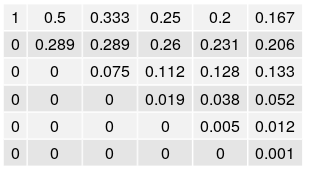
\includegraphics[]{matrizes/matriz_hilbert_CH6.png}
    \caption{Fator de Cholesky para a matriz de Hilbert com n = 6}
    \label{fig:my_label}
\end{figure}

\begin{figure}
    \centering
    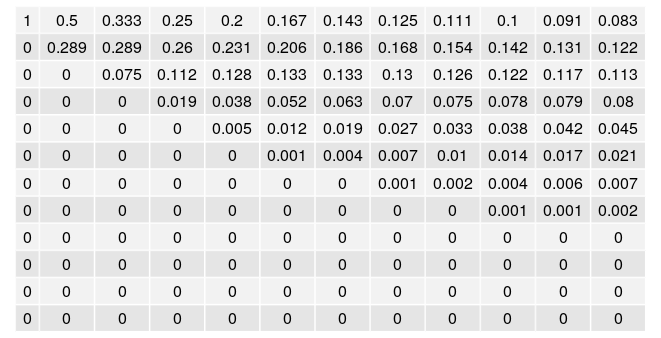
\includegraphics[width = 14.5 cm]{matrizes/matriz_hilbert_CH12.png}
    \caption{Fator de Cholesky para a matriz de Hilbert com n = 12}
    \label{fig:my_label}
\end{figure}

%comentarios%

\vspace{3mm}
\pagebreak
A seguir veremos as matrizes Q e R encontradas pela decomposição de Gram Schmidt.
Decomposição da matriz de Hilbert com Gram Schmitd para n = 2:
\begin{table}[!ht]
    \centering
\begin{minipage}[t]{0.48\linewidth}\centering
\caption{Matriz Q}
\begin{tabular}{|l|l| }
\hline
0.894 & -0.447 \\
\hline
0.447 & 0.894 \\
\hline
\end{tabular}
\end{minipage}\hfill%
\begin{minipage}[t]{0.48\linewidth}\centering
\caption{Matriz R}
\label{tab:The parameters 2 }
\begin{tabular}{|l|l|}
\hline
1.118 & 0.596 \\
\hline
0 & 0.075\\
\hline
\end{tabular}
\end{minipage}
\end{table}

Figura 3 com n = 6 e Figura 4 e 5 com n = 12
\begin{figure}[!htbp]
    \centering
    \subfloat{{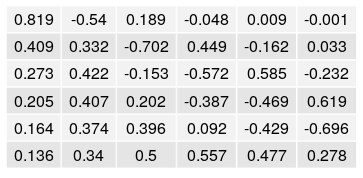
\includegraphics[width=7cm]{matrizes/matriz_hilbert_GR_Q6.png} }}
    \qquad
    \subfloat{{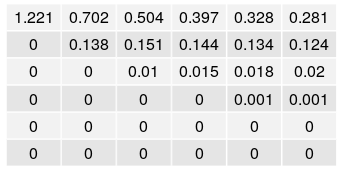
\includegraphics[width=7cm]{matrizes/matriz_hilbert_GR_R6.png} }}
    \caption{Matriz Q e R}
    \label{fig:example}
\end{figure}

\begin{figure}[!htbp]
    \centering
   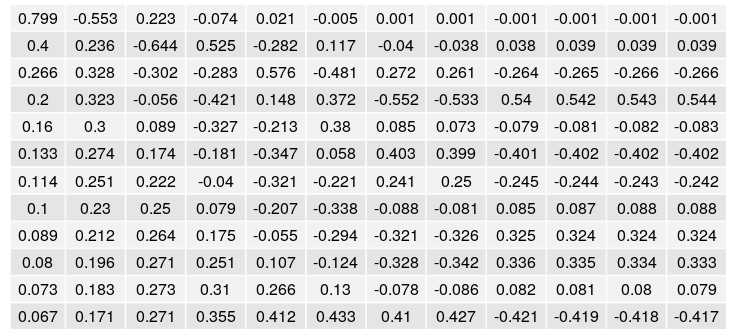
\includegraphics[width= 14.5cm]{matrizes/matriz_hilbert_GR_Q12.png}
    \caption{Saída da matriz Q com Gram Schmit para n = 12}
    \label{fig:my_label}
\end{figure}

\begin{figure}[!htbp]
    \centering
    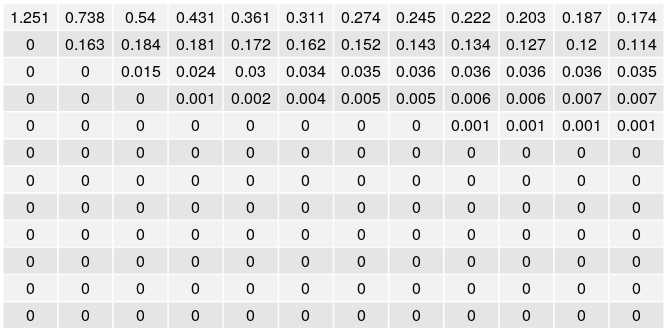
\includegraphics[width = 14.5cm]{matrizes/matriz_hilbert_GR_R12.png}
    \caption{Saída da matriz R com Gram Schmit para n = 12}
    \label{fig:my_label}
\end{figure}

%%%%%%%%%%%%%%%%%%%%%%%%%%%%%%
\newpage
A seguir veremos as matrizes Q e R encontradas pela decomposição de Householder.
Matrizes por transformação de Householder para n = 2:

\begin{table}[!htbp]
    \centering
\begin{minipage}[t]{0.48\linewidth}\centering
\caption{Matriz Q}
\begin{tabular}{|l|l| }
\hline
-0.894 & 0.447 \\
\hline
-0.447 & -0.894 \\
\hline
\end{tabular}
\end{minipage}\hfill%
\begin{minipage}[t]{0.48\linewidth}\centering
\caption{Matriz R}
\label{tab:The parameters 2 }
\begin{tabular}{|l|l|}
\hline
-1.118 & -0.596 \\
\hline
0 & -0.075\\
\hline
\end{tabular}
\end{minipage}
\end{table}

\begin{figure}[!htbp]
    \centering    \subfloat{{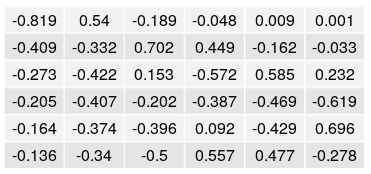
\includegraphics[width=7cm]{matrizes/matriz_hilbert_HS_Q6.png} }}
    \qquad
    \subfloat{{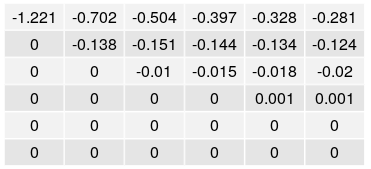
\includegraphics[width=7cm]{matrizes/matriz_hilbert_HS_R6.png}}}
    \caption{Matrizes Q e R para n=6}
    \label{fig:example}
\end{figure}
Repare que na diagonal principal de R, tanto no caso da decomposição pode Householder e Gram Schmidt, aproximamos os valores muito próximo do zero para zero. Essa aproximação não foi implementada no algoritmo, porém, tão somente para simplificação dessas imagens.

E para n = 12:
\begin{figure}[!htbp]
    \centering
    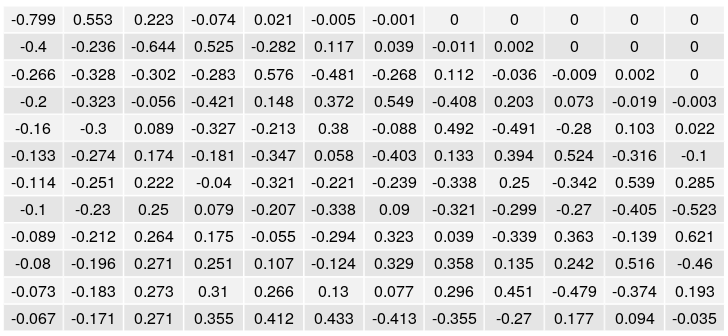
\includegraphics[width= 14.5cm]{matrizes/matriz_hilbert_HS_Q12.png}
    \caption{Saída da matriz Q para n = 12 pela decomposição de Householder}
    \label{fig:my_label}
\end{figure}
 \pagebreak
\begin{figure}[!htbp]
    \centering
    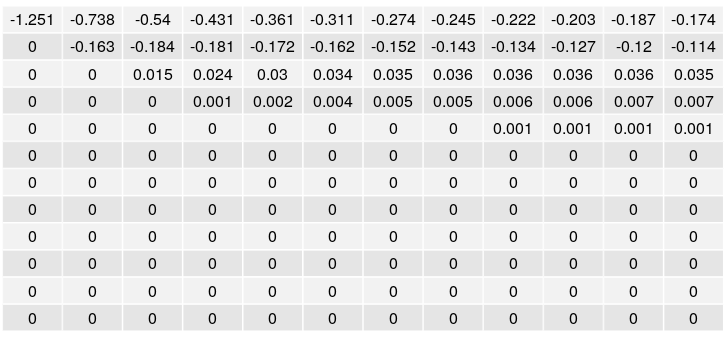
\includegraphics[width = 14.5cm]{matrizes/matriz_hilbert_HS_R12.png}
    \caption{Saída da matriz R para n = 12 pela decomposição de Householder}
    \label{fig:my_label}
\end{figure}


Primeiramente devemos observar que as decomposições QR são muito similares para quaisquer métodos utilizados, a menos dos sinais. E isso já é o esperado, pois a decomposição de QR é única se A é não singular. E a matriz de Hilbert é inversível para n arbitrário.

Ao avaliar a eficiência dos algoritimos apresentados e o condicionamento das matrizes, temos que  partir de n = 13 começamos a ter problema para encontrar o valor do condicionamento pelo método de Cholesky. E como sabemos que a matriz de Hilbert n dimensional é positiva definida \cite{song2014infinite}, estimamos, portanto, que com a propagação dos erros, a nossa matriz deixa de ser positiva definida, e consequentemente, não é possível a aplicação de tal decomposição. Todavia, os métodos de fatoração QR, uma vez que nosso estudo compreende-se por Gram Shmidt e Hourseholder, tem como principal teorema que a decomposição existe para toda matriz quadrada A, não temos o mesmo incidente de falha do método como supracitado no teorema de Cholesky.



%%%inversas




%#Comparaçoes dos metodos QR utilizando a norma1

%comparando a norma1 da matriz de hilbert com a norma dos calculos de Q*R para os metodos do refletor
% ver o valor de norma1 para cada n Norma1(matriz_de_hilbert(n)) e comparar se tem o mesmo valor para Norma1(teste_QRn)

\subsection{Inversas}
Nesta seção avaliaremos as inversas das matrizes de Hilbert que foram utilizadas para o cálculo do número de condicionamento.
Inversas das matrizes com fatoração de Cholesky, por decomposição de Householder e Gram Schmidt para n = 2 e n = 6:
\begin{table}[!htbp]
\caption{Inversa de Cholesky transposto para a matriz de Hilbert com n=2}
\centering
\begin{tabular}{|l|l|}
\hline
4 & -6  \\
\hline
-6 & 12\\
\hline
\end{tabular}
\end{table}

\begin{figure}[!htbp]
    \centering
    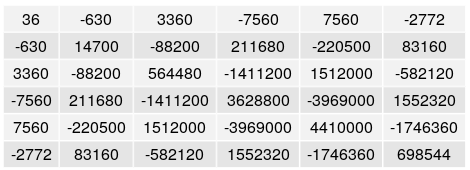
\includegraphics[]{matrizes/matriz_HINVERSA_CH6.png}
    \caption{ Inversa pelo método de Cholesky para n = 6}
    \label{fig:my_label}
\end{figure}

\begin{table}[!htbp]
\caption{Inversa por GS para a matriz de Hilbert com n=2}
\centering
\begin{tabular}{|l|l|}
\hline
4 & -6  \\
\hline
-6 & 12\\
\hline
\end{tabular}
\end{table}

\begin{figure}[!htbp]
    \centering
    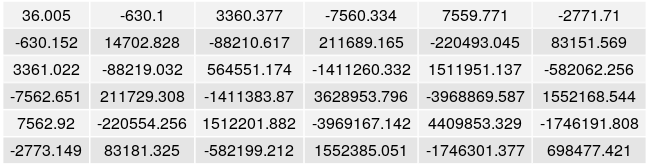
\includegraphics[width = 15cm]{matrizes/matriz_HINVERSA_GR6.png}
    \caption{Inversa por GS para a matriz de Hilbert com n = 6}
    \label{fig:my_label}
\end{figure}

\begin{table}[!htbp]
\caption{Inversa da matriz por tranformação de Householder para n=2}
\centering
\begin{tabular}{|l|l|}
\hline
4 & -6  \\
\hline
-6 & 12\\
\hline
\end{tabular}
\end{table}


\begin{figure}[!htbp]
    \centering
    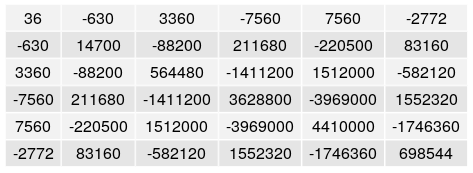
\includegraphics[]{matrizes/matriz_HINVERSA_HH6.png}
    \caption{Inversa da matriz por tranformção de Householder para n = 6}
    \label{fig:my_label}
\end{figure}

\newpage

Após a elaboração das inversas das matrizes para cada método, com n= 2 e 6, observa-se que para n=2 os três métodos têm exatamente a mesma matriz, entretanto, para n=6, a matriz da inversa de Cholesky e Householder são as mesmas, enquanto a de Gram Schmidt tem pequenas variações nas casas decimais. Isso se deve ao fato, como já citado anteriormente, de tal método ser instável numericamente, já que quando o executamos em um computador, os vetores não ficam tão bem ortogonalizados devido a erros de ponto flutuante.


Verificando os códigos na seção de anexo, pode-se verificar o procedimento da comparação entre a norma da matriz de Hilbert para n = 2, 6, 12, 20 e a norma da fatoração QR tanto para o método de Gram Schmidt como o de Householder para os mesmos tamanhos de n.  Isto é, comparamos a norma da matriz de Hilbert original, com a matriz aproximada, obtida através da multiplicação de QR das decomposições utilizadas. Observando os resultados, temos como conclusão que tais comparações mostram que as normas possuem o mesmo valor. 

Sendo assim, avaliamos que o método de decomposição QR foi bastante eficaz, uma vez que estamos reobtendo matrizes com valores muito próximos da matriz original.
Entretanto, se aumentassemos a precisão da norma para um número muito maior de casas decimais, estimamos que veríamos alguma diferença. 

\subsection{Condicionamento}

Quando tratamos de número de condicionamento, avaliamos se a matriz tem boas condições de ser tratada numericamente. Isto é, avaliamos a sensibilidade dos valores da solução x de um sistema através de mudanças nos valores de entradas b (Ax = b). Temos que, ao calcular o número do condição de determinada matriz, a mesma estará bem condicionada se o número calculado for pequeno, e mal condicionada, caso contrário. Quando estudamos o número de condição associado a uma matriz $A$ de um sistema linear $Ax = b$, tal número, nos retorna como a solução do sistema x se comporta para variações da matriz b.


Em nosso caso de estudo, para calcularmos o número de condicionamento em todos os métodos para cada n, usamos a norma 1, onde realizamos a norma da matriz de hilbert inversa calculada em cada um dos métodos, multiplicado pela norma da matriz de Hilbert.

\begin{equation}
    \kappa_1(A) = ||A||_1 ||A^{-1}||_1
\end{equation}

Para o cálculo da matriz de Hilbert inversa implementamos os algoritmos de substituição direta e retrosubstituição e encontramos a solução para o seguinte sistema:
AX = I em que I era uma matriz Identidade de dimensão n e A a matriz de Hilbert de dimensão n. Logo, através da fatoração de Cholesky, reduzimos o problema a $R^{T}RX = I$ que implicou na solução usual por Cholesky que é resolver os dois problemas seguintes:
\begin{equation}
    R^{T}Y = I 
\end{equation}

\begin{equation}
    RX = Y
\end{equation}
em que R é o fator de Cholesky.

Já para os casos de decomposição QR, fizemos algo semelhante, encontramos a inversa da matriz de Hilbert de dimensão n resolvendo o seguinte sistema:

\begin{equation}
   RX = Q^{T}I
\end{equation}
em que Q e R são encontradas através de uma das decomposições utilizadas, sendo Q uma matriz ortogonal e R uma matriz triangular superior de dimensões n.

Após a realização do cálculo, oberservamos que para n=2, os três métodos têm o mesmo número de condicionamento que é igual a 27 e para n=6 o método de Cholesky e Householder também possuem o mesmo número, igual a 29.070.279 enquanto Gram-Schmidt teve uma pequena variação de 960 (sendo de 29.071.239). Todavia, temos que para n=12 em Cholesky e Householder o número de condicionamento possui um valor muito superior do que a Gram-Schmidt, e assim, consequentemente, para n=20, o condicionamento calculado através de Householder comparado a Gram-Schmidt continua crescendo com uma taxa muito mais elevada. 
Então, para n = 11, encontramos para Householder o número de condicionamento igual a $1,23.10^{15}$ e pela fatoração de Cholesky obtivemos $\kappa_1 = 1,27.10^{15}$, enquanto que por Gram-Schmidt obtivemos um número relativamente baixo de $1,21.10^{9}$.

Por fim, observamos novamente que o número de condição na aplicação de Gram Schmidt para cálculo da inversa de A, em nosso estudo,  não explode como nos outros dois métodos, sendo assim, extraímos de tal avaliação, que o método em questão é melhor condicionado do que os outros também analisados. 
Não obstante, a avaliação supracitada, diverge com as análises da literatura, uma vez que, contrariamente, é dito que o método de Gram Schmidt é deveria resultar em um pior condicionamento comparado a Householder, já que para dimensões grandes, deveria ocorrer um erro de ortogonalização dos vetores de A. Em investigações realizadas dentro do nosso estudo, suspeitamos que essa contrariedade em questão, pode vir da liguagem RStudio utilizada, - que poderia estar propagando mais erros em alguma de nossas operações em Householder, ou ainda, algum comando utilizado, onde também poderia estar propiciando tal questão.

\subsection{Estimativa do Condicionamento}

Além de toda discussão acima, neste trabalho, também fizemos duas estimativas para o número de condicionamento da matriz de Hilbert. As duas estimativas podem ser encontradas em Watkins(2004).
Pelo teorema 2.2.25 do livro do Watkins, vemos que:
\begin{equation}
    \kappa_1(A) \geq \frac{||a_i||_1}{||a_j||_1}
\end{equation}

Desde que A seja não singular, a relação vale para qualquer i e j, tais que, $a_1, a_2,... $ sejam às colunas da matriz A. Neste projeto, como já vimos anteriormente, fizemos a decomposição da matriz A nas componentes Q e R, portanto, para a estimativa do número de condicionamento encontramos um A aproximado através da multiplicação de Q por R e através de nossas implementações, calculamos o limitante inferior para o condicionamento.

Para esta primeira estimativa, o limitante inferior do número de condicionamento foi deveras pequeno, para uma matriz de Hilbert de dimensão 10, foi encontrado o valor de 28 para quaisquer métodos. Valor muito inferior ao calculado para o número de condicionamento nas outras seções do trabalho.


Também fizemos uma segunda estimativa usando o teorema 2.2.28 do livro do Watkins, temos então que:
\begin{equation}
    \kappa_1(A) \geq \frac{||A||_1 ||A^{-1}w||_1}{||w||_1}
\end{equation}

Nessa estimativa, temos que $w \in R^{n}$ qualquer, desde que $w$ seja não nulo. Em nosso algoritmo, usamos um vetor de tamanho n de entradas todas 1.
Essa estimativa, também ficou muito abaixo dos valores de condicionamentos encontrados no restante do trabalho, sendo o valor encontrado para uma matriz de Hilbert de dimensão 10 de somente 7 milhões usando quaisquer métodos, sendo muito menor do que o valor de condicionamento encontrado para a matriz de mesma dimensão no restante do trabalho. Portanto, julgamos que essa foi uma estimativa ruim.
\printbibliography
\nocite{watkins2004fundamentals}
\nocite{lopes1996calculo}
\nocite{strang1993introduction}

\newpage
\section{Anexos}

\begin{lstlisting}
matriz_de_hilbert <- function(n){ #Gera uma matriz de Hilbert de dimensão n
  
  H <- matrix(0, n, n) 
# n e o tamanho da matriz (quadrada) 
# matriz H (matriz de hilbert)
  
  for(i in 1:n){
   for(j in 1:n){
     H[i,j] <- (1/(i+j-1))
     
    }
  }
 return(H)
}

matriz_Identidade <- function(n){ #Gera uma matriz de Identidade de dimensão n
  
  I <- matrix(0, n, n) 
# n e o tamanho da matriz (quadrada) 
# matriz I (matriz Identidade)
  
  for(i in 1:n){
   for(j in 1:n){
     if(i == j){
     I[i,j] <- 1
     }
    }
  }
 return(I)
}

fator_cholesky <- function(A){ #Encontra o fator de Cholesky
  #preciso do pacote Matrix para rodar alguns comandos
  require(Matrix)
  library("Matrix")
  
  #transformando A numa classe de matriz
  A <- as.matrix(A)
  #n e o numero de colunas que tem na matriz A
  n <- ncol(A)

  #matriz quadrada definida positiva numero de colunas = numero de linhas
  #inicializando a matriz Rt, que e a transposta da matriz R
  Rt <- matrix(0,n, n)

  #posso usar o comando do R: chol(A) para testar se esta certo meu codigo e se a matriz e definida positiva, se nao for o comando
  #chol(A) retornara um erro acusando que a matriz nao e definida positiva
  
  #fatoracao de cholesky   
  if(n > 0){
    for (i in 1:n) {
      for (j in 1:i){
        soma <- 0
        for(k in 1:j){
          # %*% realiza o produto interno
          soma <- (soma + Rt[i,k] %*% Rt[j,k])
        }
        #se A[i,i] <= 0 a matriz nao e difinida positiva(definicao do watkins algoritmo 1.4.17)
        if(A[i,i] < 0 || A[i,] == 0){
          return("matriz nao e definida positiva") 
          break
        }
        if(i==j){
          #calculo das diagonais
          Rt[i,j] <- sqrt(A[i,i] - soma)
        }else{
          #calculo das outras posicoes 
          Rt[i,j] <- (A[i,j] - soma) / Rt[j,j]
        }
      }
    }  
  }
  R <- t(Rt)
  #retorna a matriz transposta de R que e uma triangular inferior
  return(R)
}

qr.gramschmidt <- function(A){ #Decomposição QR por GS
  require(Matrix)

Q <- as.matrix(A) #Comeca com Q = A

n <- ncol(A)
m <- nrow(A)

R <- matrix(0, n, n) #Comeca R

for (k in 1:n){
  v = A[,k] #vetores colunas de A
   if (k > 1) { #pula quando k=1
    for (c in 1:(k-1)) {
     R[c,k] <-  A[,k] %*% Q[,c] #produto interno
    
     v <- v -  R[c,k] * Q[,c]  
    }      
}
  R[k,k] <- sqrt(sum(v^2))
  Q[,k] <- v / R[k,k]
}

res <- list('Q'=Q,'R'=R)
return(res)
}

#Esta função faz a transofrmação QR da matriz A pelo método de Householder.
#O argumento de entrada é a matriz A e a função retorna uma lista com as matrizes Q e R
#Ideia do algoritmo: A ideia do algoritmo é, dada a matriz A, obter o seu posto (o menor valor dentre número de linhas e colunas) e obter todas as Qs utilizando a matriz identidade e o vetor alvo (vetor u (coluna da matriz A da qual queremos zerar os elementos)). Por fim, a Q é obtida multiplicando as Qs anteriores e R é obtido no produto matricial de Q com A.
qr.householder <- function(A){
  require(Matrix)
  
  R <- as.matrix(A) #Comeca com R = A
  
  n <- nrow(A)
  m <- ncol(A)
  H <- list() #A lista H vai armazenar as Q's
  
  if (n > m) { #posto de A
    p <- m
  } else {
    p <- n
  }
  
  for (k in 1:p) {
    x <- R[k:n,k] #Vetor alvo
    e <- as.matrix(c(1, rep(0, length(x)-1))) #replica o valor 
    v <- sign(x[1]) * sqrt(sum(x^2)) * e + x #vetor v
    
    u <- v / sqrt(sum(v^2)) #normalizacao de v
    
    #Achando matriz Qk
    Qk <- diag(length(x)) - 2 * as.vector(u %*% t(u)) 
    if (k > 1) { #Para os vetores alvos a partir do 2
      Qk <- bdiag(diag(k-1), Qk) #devemos acrescentar linhas para a mesma dimensao de A, criando matriz diagonal em bloco. Constrói uma matriz diagonal esparsa, unindo várias matrizes em bloco.
    }
    
    #Armazenando as Q's
    H[[k]] <- Qk
    
    R <- Qk %*% R #obtendo R
  }

  Q <- Reduce("%*%", H) #Obtendo Q multiplicando todas as Q's
  res <- list('Q'=Q,'R'=R)
  return(res)
}

#Resolver o sistema Rt*Y = matriz B por substituicao direta

substituicao_direta <- function(Rt, B){
  
  #n e o numero de colunas que tem na matriz Rt
  n <- ncol(Rt)

  #inicializando a matriz Y
  Y <- matrix(0,n)
  for (i in 1:n){
    soma <- 0
    for (j in 1:n){
      if (i == j){
        #calculo da matriz Y
        Y[i] <- (B[i] - soma)/Rt[i,j]
        break
      } 
      else{
        soma <- soma + (Rt[i,j] %*% Y[j])
      }  
    }    
  }
  #retorna os valores da matriz Y
  return(Y)
}    


 #Resolver o sistema R*x = Y 
 #R e uma triangular superior
 #R e o fator de cholesky
 #posso usar o comando backsolve(t(Rt),Y) para testar se esta certo, onde t(Rt) = R

retrosubstituicao <- function(Rt,Y){
  
  R <- Rt
  #n e numero de colunas de R
  n <- ncol(R)
  
  #inicializando o vetor X
  X <- matrix(0,n)

  #valor da ultima posicao do vetor X
  X[n] <- Y[n]/R[n,n] 
  
  for (i in (n-1):1){
    soma <- 0
    for (j in (i+1):n){
      soma <- soma + (R[i,j] %*% X[j])
    }
    X[i] <- (Y[i] - soma)/R[i,i]
  }  
  
  #retorna os valores do vetor X
  return(X)
}
#Calcula a inversa da matriz A sem decomposição, não foi usado no nosso código, mas foi implementado para fins de comparação
Inversa <- function(A){
  n <- ncol(A)
  X <- matrix(0,n,n)
  for(i in 1:n){
    X[,i] <- cbind(substituicao_direta(A, matriz_Identidade(n)[,i]))
  }
  return(X)
}    

#Realiza a operação de encontrar a inversa de qualquer matriz A através da decomposição de Cholesky, no nosso caso, calcula a inversa da matriz de Hilbert de dimensão n
Inversa_por_Cholesky<- function(A){
  n <- ncol(A)
  R <- matrix(0,n,n)
  Y <- matrix(0,n,n)
  X <- matrix(0,n,n)
   R <- fator_cholesky(A)
   

  for(i in 1:n){
   Y[,i] <- cbind(substituicao_direta(t(R), matriz_Identidade(n)[,i])) #Resolve o sistema linear através da fatoração de Cholesky (A = Rt*R) Rt*Y = B 
  }
  for(i in 1:n){
    X[,i] <- cbind(retrosubstituicao(R, Y[,i])) #R*X = B, B é a matriz Identidade e encontramos X = a inversa de A
  }
  return(X)
}    

#Realiza a operação de encontrar a inversa de qualquer matriz A através da decomposição de Gram-Schmidt, no nosso caso, calcula a inversa da matriz de Hilbert de dimensão n
Inversa_por_QR_GS<- function(A){
  n <- ncol(A)
  Q <- matrix(0,n,n)
  R <- matrix(0,n,n)
  Y <- matrix(0,n,n)
  X <- matrix(0,n,n)
  Q <- qr.gramschmidt(A)$Q
  R <- qr.gramschmidt(A)$R

  Y <- t(Q) %*% matriz_Identidade(n) #Faz Qt*B
   
  for(i in 1:n){
    X[,i] <- cbind(retrosubstituicao(R, Y[,i])) #Resolve o sistema linear através da decomposição QR (A = Q*R) R*X = Qt*B 
  }
  return(X)
}

#Calcula a norma 1 da matriz A

 Norma1 <- function(A){
  n <- ncol(A)
  Y <- matrix(0,n)
  for (i in 1:n){
    soma <- 0
    for(j in 1:n){
      soma <- soma + (abs(A[j,i]))
    }
    Y[i] <- soma
  }
  x <- max(Y)
  return(x)
}

#Calcula o número de condicionamento multiplicando a norma 1 de A e a norma 1 da inversa de A (A^-1)

cond <- function(x,y){
  cond <- x*y
  return(cond)
}

#Calcula a norma de A^-1*w e divide pela norma de w, w vetor qualquer, no caso o vetor com todas entradas 1

estimativa1 <- function(Y){
  n <- ncol(Y)
  Y <- matrix(0,n,n)
  w <- seq(1,n)
  for(i in 1:n){
    w[i] <- 1
  }
  norma_um <- sum(abs(w))
  soma <- sum(abs(Inversa_por_Cholesky(matriz_de_hilbert(n))%*%w))
  v <- soma/norma_um
  print(v)
}


#Estimativa do limitante inferior do número de condicionamento de A, através de Q*R

estimativa2 <- function(x,v){
  estimativa2 <- x*v
  return(estimativa2)
  }
  
#Estimativa do limitante inferior do número de condicionamento de A, através de A = Q*R, olhamos a maior norma de qualquer coluna de A e dividimos pela menor norma das colunas de A = Q*R

estimativa3 <- function(A){
  n <- ncol(A)
  X <- matrix(0,n,n)
  X <- A
  C <- matrix(0,n,n)
  D <- matrix(0,n,n)
  soma1 <- 0
  soma2 <- 0
  for(j in 1:n){
   for(i in 1:n){
   soma1 <- soma1 + sum(abs(A[i,1]))
   }
    C[j] <- soma1
  }
  for(j in 1:n){
   for(i in 1:n){
  soma2 <- soma2 + sum(abs(A[i,2]))
   }
    D[j] <- soma2
  }
  c <- max(C[,1])/min(D[,1])
  print(c)
}


\end{lstlisting}


\end{document}